\label{dev}

The POP model (chapter \ref{popmodel}) is a suitable programming model for large heterogeneous distributed environments but it should also remain as close as possible to traditional object oriented programming. Parallel objects of the POP model generalize sequential objects, keep the properties of object oriented programming (data encapsulation, inheritance and polymorphism) and add new properties.\s

The POP-Java language is an extension of Java that implements the POP model. Its syntax remains as close as possible to standard Java so that Java programmer can easily learn it and existing Java libraries can be parallelized without much effort. Changing a sequential Java application into a distributed parallel application is rather straightforward. POP-Java is also very close to POP-C++ so that POP programmer can use both system easily.\s

Parallel objects are created using parallel classes. Any object that instantiates a parallel class is a parallel object and can be executed remotely. To help the POP-C++ runtime to choose a remote machine to execute the remote object, programmers can add object description information to each constructor of the parallel object. In order to create parallel execution, POP-Java offers new semantics for method invocations. These new semantics are indicated thanks to new POP-Java keywords. This chapter describes the syntax of the POP-Java programming language and presents the main tools available in the POP-Java system.


\subsection{Parallel objects}
POP-Java parallel objects are a generalization of sequential objects. Unless the term sequential object is explicitly specified, a parallel object is simply referred as an object in the rest of this chapter.

\subsubsection{Create a parallel class}
Developing POP-Java application mainly consists of designing an implementing parallel classes.
The declaration of a parallel class is the same as a standard Java class declaration, but it has to be annotated
with the annotation \textbf{@POPClass}.
The parallel class can extend another parallel class but not a sequential class.\s

\textbf{Simple parallel class declaration}
\begin{lstlisting}
@POPClass
public class MyParallelClass {
	//Implementation
}
\end{lstlisting}\s

\textbf{Parallel class declaration with an inheritance}
\begin{lstlisting}
@POPClass
public class MyParallelClass extends AnotherParallelClass {
	//Implementation
}
\end{lstlisting}\s

As Java allows only the single inheritance, a parallel class can only inherit from \textbf{one} other parallel class.
The Java language also impose that the file including the parallel class has the same name than the parallel class.\s

POP-Java imposes also one restrictions. The parallel class must be declared and implemented in a file with \textbf{.pjava} extension.
For example, the parallel class \textit{MyParallelClass} declared before, must be in a file \textbf{MyParallelClass.pjava}.\s

Parallel classes are very similar to standard Java classes. As POP-Java has some different behavior, some restrictions applied to the parallel classes : 
\begin{itemize}
\item All attributes in a parallel class must be protected or private
\item The objects do not access any global variable
\item A parallel class does not contain any static attributes or static methods
\end{itemize}


\subsubsection{Creation and destruction}
The object creation process consists of several steps: locating a resource satisfying the object description (resource discovery), transmitting and executing the object code, establishing the communication, transmitting the constructor arguments and finally invoking the corresponding object constructor. Failures on the object creation will raise an exception to the caller. Section \ref{exception} will describe the POP-Java exception mechanism.\s

As a parallel object can be accessible concurrently from multiple distributed locations (shared object), destroying a parallel object should be carried out only if there is no other reference to the object. POP-Java manages parallel objects' life time by an internal reference counter. A counter value of 0 will cause the object to be physically destroyed. \s

Syntactically, the creation of a parallel object is identical to the one in Java. A parallel object can be created by using the standard new operator of Java.


\subsubsection{Parallel class methods}
Like sequential classes, parallel classes contain methods and attributes.
Method can be public or private but attribute must be either protected or private.
For each public method, the programmer must define the invocation semantics.
These semantics, described in section \ref{semantic}, are specified by an annotations.

\begin{itemize}
\item \textbf{Interface side} : These semantics affect the caller side.
\subitem sync : Synchronous invocation. 
\subitem async : Asynchronous invocation.
\item \textbf{Object side} : These semantics affect the order of the class inside the object itself.
\subitem seq : Sequential invocation
\subitem conc : Concurrent invocation
\subitem mutex : Mutual exclusive invocation
\end{itemize}

The combination of the interface and object-side semantics defines the overall semantics of a method. There
are 6 possible combinations of the interface and object-side semantics, resulting in 6 annotions:

\begin{lstlisting}
@POPSyncConc
@POPSyncSeq
@POPSyncMutex
@POPAsyncConc
@POPAsyncSeq
@POPAsyncMutex
\end{lstlisting}
\pagebreak
For example, a synchronous concurrent method returning an int value must be declared as follow : 
\begin{lstlisting}
@POPSyncConc
public int myMethod(){
	return myIntValue;
}
\end{lstlisting}

A method declared as asynchronous must have its return type set to void. Otherwise, the compiler will raise an error.


\subsubsection{Object description}
\label{dev:objdesc}
Object descriptions are used to describe the resource requirements for the execution of an object.
Object descriptions are declared along with parallel object constructor declarations.
The object description can be declared in a static way as an annotation of the constructor, or in a dynamic way
as an annotation on the parameters of the constructor. First an example of a static annotation:

\begin{lstlisting}
@POPObjectDescription(url="localhost")
public MyObject(){
}
\end{lstlisting}\s

and now a dynamic example:
\begin{lstlisting}
public MyObject(@POPConfig(Type.URL) String host){
}
\end{lstlisting}\s

Currently only the url annotation is implemented, allowing to specify the url/IP of the machine on which the POP-Object is executed.
If the annotation is not set, POP-Java will use the POP-C++ jobmanager to find a suitable machine.

\begin{comment}
Here are the list of accepted resource requirements expressions in the current POP-Java version : 

\begin{itemize}
\item od.power(exact, lbound) : Specify the computing power needed (in Mflops).
\item od.memory(exact, lbound) : Specify the memory size needed (in MB).
\item od.bandwidth(exact, lbound) : Specifiy the bandwidth (in Mb/s) needed for the connection.
\item od.encoding(string) : Specify the encoding ("raw" or "xdr") used for the data transfer.
\item od.protocol(string) : Specify the protocol (only "socket" for the moment) used for the network connection.
\end{itemize}

Both \textit{exact} and \textit{lbound} terms are numeric expressions and \textit{string} is a standard Java string expression.
The object descriptions allowing two values (\textit{exact} and \textit{lbound}) have a priority set to the first value.
If no resource are found for this specified \textit{exact} value, the \textit{lbound} value will be used.\s

An example of object description is given in the following code.
The constructor for the parallel object \textit{MyParallelClass} requires the computing power of "p" Mflops or at least 80 Mflops.
The memory requirement is set to 100MB or at least 60MB.


\begin{lstlisting}
public parclass MyParallelClass {
	public MyParallelClass(float p) @{ od.power(p, 80); 
	  od.memory(100,60); }{
		
	}
}
\end{lstlisting}\s



The object description are used by the POP-C++ runtime system to find suitable resource for executing the parallel object.
Matching between object descriptions and resources is carried out by a multi-layer filtering technique: first, each expression (item) in every object descriptor will be evaluated and categorized (e.g., power, memory, network).
Then, the matching process consists of several layers: each layer filters single category within the object descriptors and performs matching on that category. Finally, if an object descriptor pass all filters, the object is assigned to that resource.\s

If no suitable resource is found to execute the object then an exception is raised.
\end{comment}

\subsubsection{Data marshaling and IPOPBase}
When calling a remote methods, the arguments must be transferred to the object being called (the same happens for the return value and the exception).  In order to operate with different memory spaces and different architecture, data is marshaled into a standard format prior to be send to remote objects. All data passed is serialized (marshaled) at the caller side an deserialized (unmarshaled) at the called side. \s

With POP-Java all primitive types, primitive types arrays and parallel classes can be passed without any trouble to another parallel object. This mechanism is transparent for the programmer.\s

If the programmer want to pass a special object to or between parallel classes, this object must implement the IPOPBase interface from the POP-Java library. This library is located in the installation directory (\textit{POPJAVA\_LOCATION/JarFile/popjava.jar}). By implementing this interface, the programmer will have to override the two following methods : 

\begin{lstlisting}
@Override
public boolean deserialize(Buffer buffer) {
  return true;
}

@Override
public boolean serialize(Buffer buffer) {
  return true;
}
\end{lstlisting}\s

These methods will be called by the POP-Java system when an argument of this type need to be serialized or deserialized. As the object will be reconstruct on the other side and after the values will be set to it by the deserialize method, any class implementing the IPOPBase interface must have a default constructor.\s

\pagebreak
The code below shows a full example of a class implementing the IPOPBase interface.


\begin{lstlisting}
import popjava.buffer.Buffer;
import popjava.dataswaper.IPOPBase;

public class MyComplexType implements IPOPBase {
	private int theInt;
	private double theDouble;
	private int[] someInt;
	
	public MyComplexType(){}
	
	public MyComplexType(int i, double d, int[] ia){
		theInt = i;
		theDouble = d;
		someInt = ia;
	}
	
	@Override
	public boolean deserialize(Buffer buffer) {
		theInt = buffer.getInt();
		theDouble = buffer.getDouble();
		int size = buffer.getInt();
		someInt = buffer.getIntArray(size);
		return true;
	}

	@Override
	public boolean serialize(Buffer buffer) {
		buffer.putInt(is);
		buffer.putDouble(ds);
		buffer.putIntArray(ias);		
		return true;
	}
}
\end{lstlisting}

\subsection{POP-Java behavior}
This section aims to explain to difference between the standard Java behavior and the POP-Java behavior.\s

As in standard Java, the primitive types will not be affected by any manipulations inside a methods. The objects will be affected only if the method semantic is “Synchronous”. In fact, POP-Java serialize the method arguments to pass them on the object-side. Once the method work is done, the arguments are serialize once again to be send back to the interface-side. If the method semantic is “Synchronous”, the interface-side will deserialize
the arguments and replace the local ones by the deserialized arguments. If the method semantic is
“Asynchronous”, the interface-side will not wait for any answer from the object-side. It's important to understand this small difference when developing POP-Java application.

\subsection{Exception handling}
\label{exception}
Errors can be efficiently handled using exceptions. Instead of handling each error separately based on an error code returned by a function call, exceptions allow the programmer to filter and centrally manage errors trough several calling stacks. When an error is detected inside a certain method call, the program can throw an exception that will be caught somewhere else.\s

The implementation of exception in non-distributed applications, where all components run within the same memory address space is fairly simple. The compiler just need to pass a pointer to the exception from the place where it is thrown to the place where it is caught.  However, in distributed environments where each component is executed in a separated memory address space (and eventually data are represented differently due to heterogeneity), the propagation of exception back to a remote component is complex.

\begin{figure}[ht]
\caption{Exception handling example}
\center
\label{fig:exception}
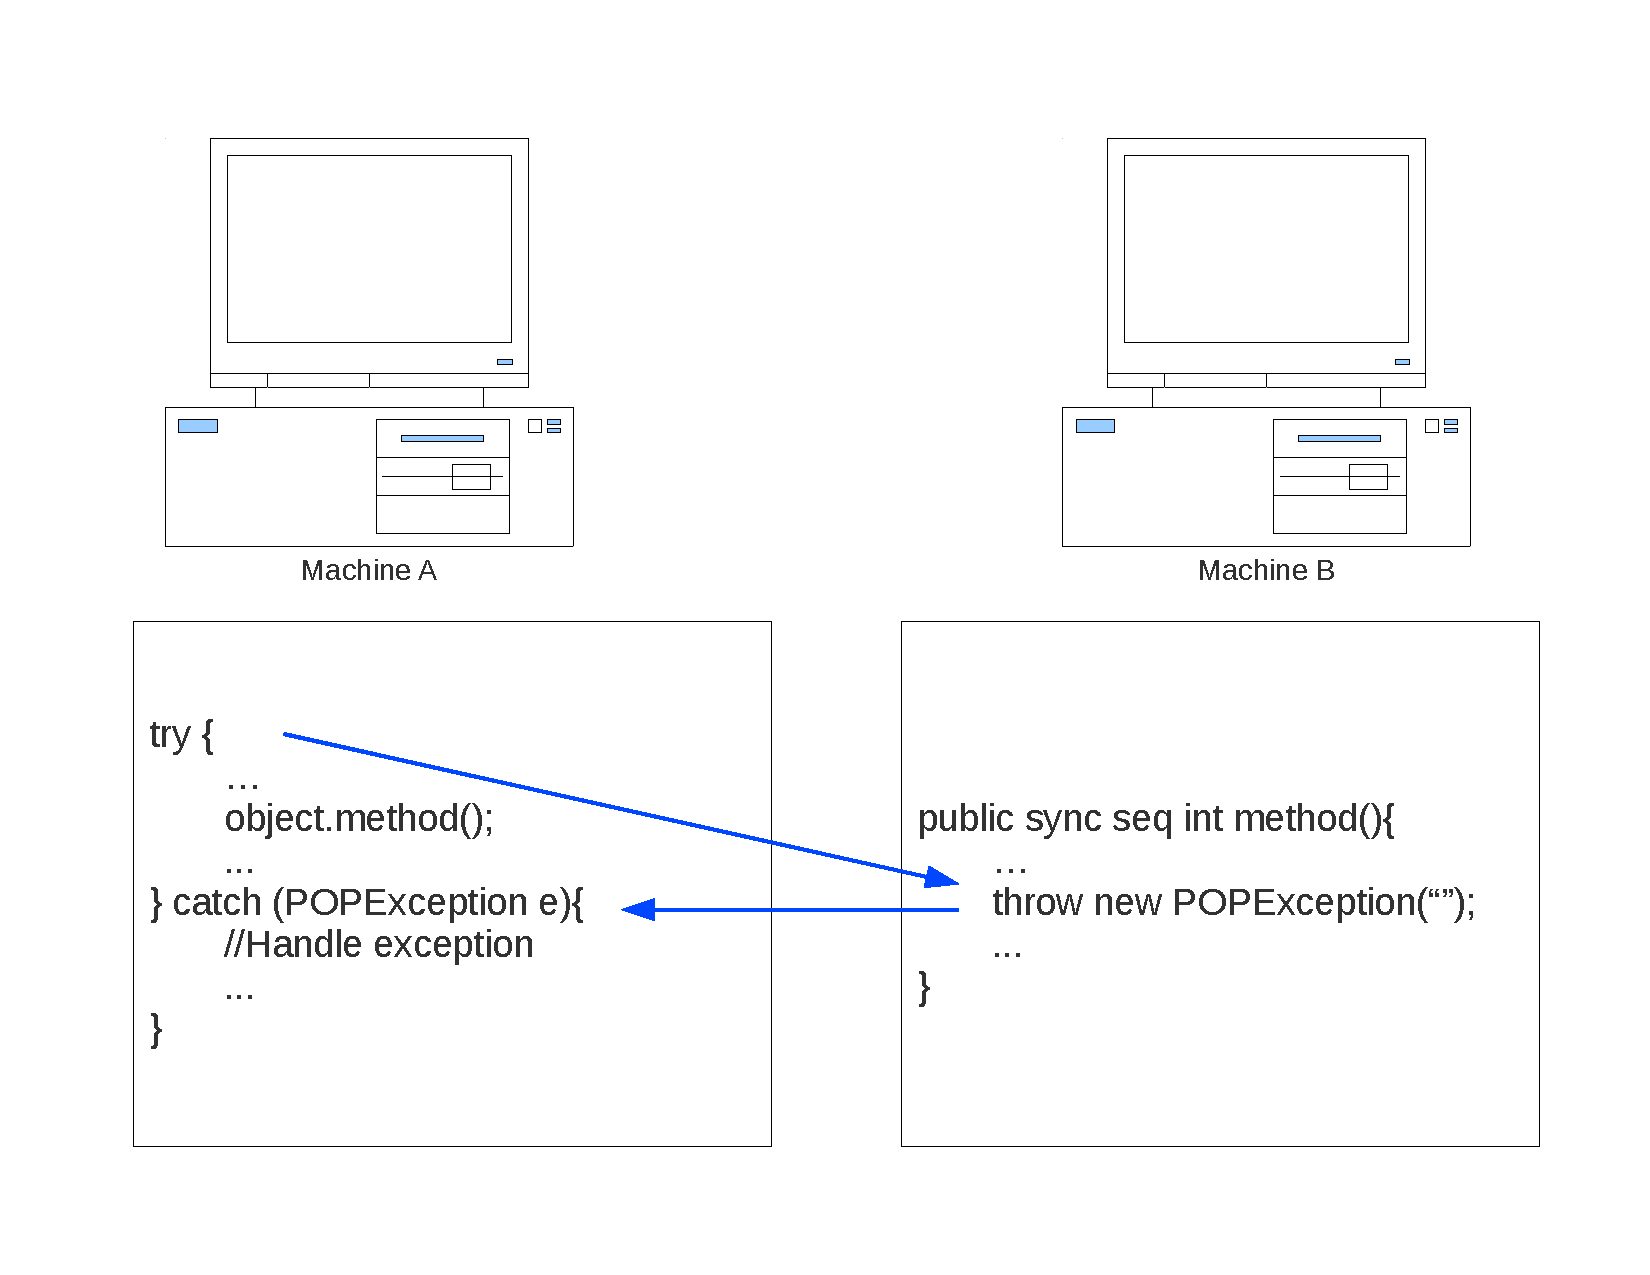
\includegraphics[scale=0.3]{exception.pdf}
\end{figure}

POP-Java supports transparent exception propagation. Exceptions thrown in a parallel object will be automatically propagated back to the remote caller (figure[\ref{fig:exception}]). The current POP-Java version allows the following types of exceptions : 
\begin{itemize}
\item Exception
\item POPException
\end{itemize}

The invocation semantics of POP-Java affect the propagation of exceptions. For the moment, only synchronous methods can propagate the exception. Asynchronous methods will not propagate any exception to the caller. POP-Java current behavior is to abort the application execution when such exception occurs. 


